\section{後処理と描画} \label{sec:ideal_exp_sno}
%------------------------------------------------------
ここでは後処理と計算結果の描画方法を説明する。このチュートリアルでは、
{\netcdf}形式の分散ファイルを単一のファイルに結合し、\grads でも読み込み可能な{\netcdf}形式に変換する。
まず、\ref{sec:compile_sno}節でコンパイルした後処理ツール\sno へのリンクを張る。
\begin{verbatim}
  $ ln -s ../../../../bin/sno  ./
\end{verbatim}

\sno の実行方法は、基本的に{\scalerm}と同じであり、
\begin{verbatim}
  $ mpirun  -n  [プロセス数]  ./sno  [設定ファイル]
\end{verbatim}
の形式で実行する。
\verb|sno_R20kmDX500m.conf|は\sno 専用の設定ファイルである。
この設定ファイルを\sno に与えて、次のように実行する。
\begin{verbatim}
  $ cp  sample/sno_R20kmDX500m.conf  ./sno_R20kmDX500m.conf
  $ mpirun  -n  2  ./sno  sno_R20kmDX500m.conf
\end{verbatim}
エラーメッセージがなく、下記のメッセージだけが標準出力へ表示されていれば、変換は正常に完了している。
\msgbox{
\verb|*** End   SCALE-NetCDF Operator| \\
}

\sno 実行時のプロセス数は、1領域に含まれる\texttt{HALO}領域を除いた格子点数の約数でなければならない。
%HDDの読み書き速度に依存するが、本書の必要要件にあった計算機であれば2分程度で計算が終わる。
この実行によって、実行ディレクトリ下に下記のファイルが作成される。
\begin{alltt}
  merged_history.pe000000.nc
\end{alltt}
このNetCDFファイルは、\grads のsdfopen関数を用いて読み込むことが可能なNetCDFファイルである。
自己記述形式で自分自身が軸情報等、\grads の描画に必要な要素を持っており、ctlファイルがなくても読み込むことができる。

計算が問題なく完了しているかを確認するため、\grads スクリプト \verb|checkfig_ideal.gs|
を使って作図する。なお、\grads のバージョンによって文法が異なるため、
警告が出る場合には\grads スクリプトを適宜変更されたい。
作図は以下のコマンドで行う。
\begin{verbatim}
  $ grads -blc checkfig_ideal.gs
\end{verbatim}
コマンドが成功すれば、下記のファイルが生成される。
\begin{verbatim}
   ideal_qhyd.png
   ideal_W.png
\end{verbatim}
シミュレーションと後処理が問題なく行われていれば、図\ref{fig_ideal}と同じ図が得られる。

\begin{figure}[t]
\begin{center}
  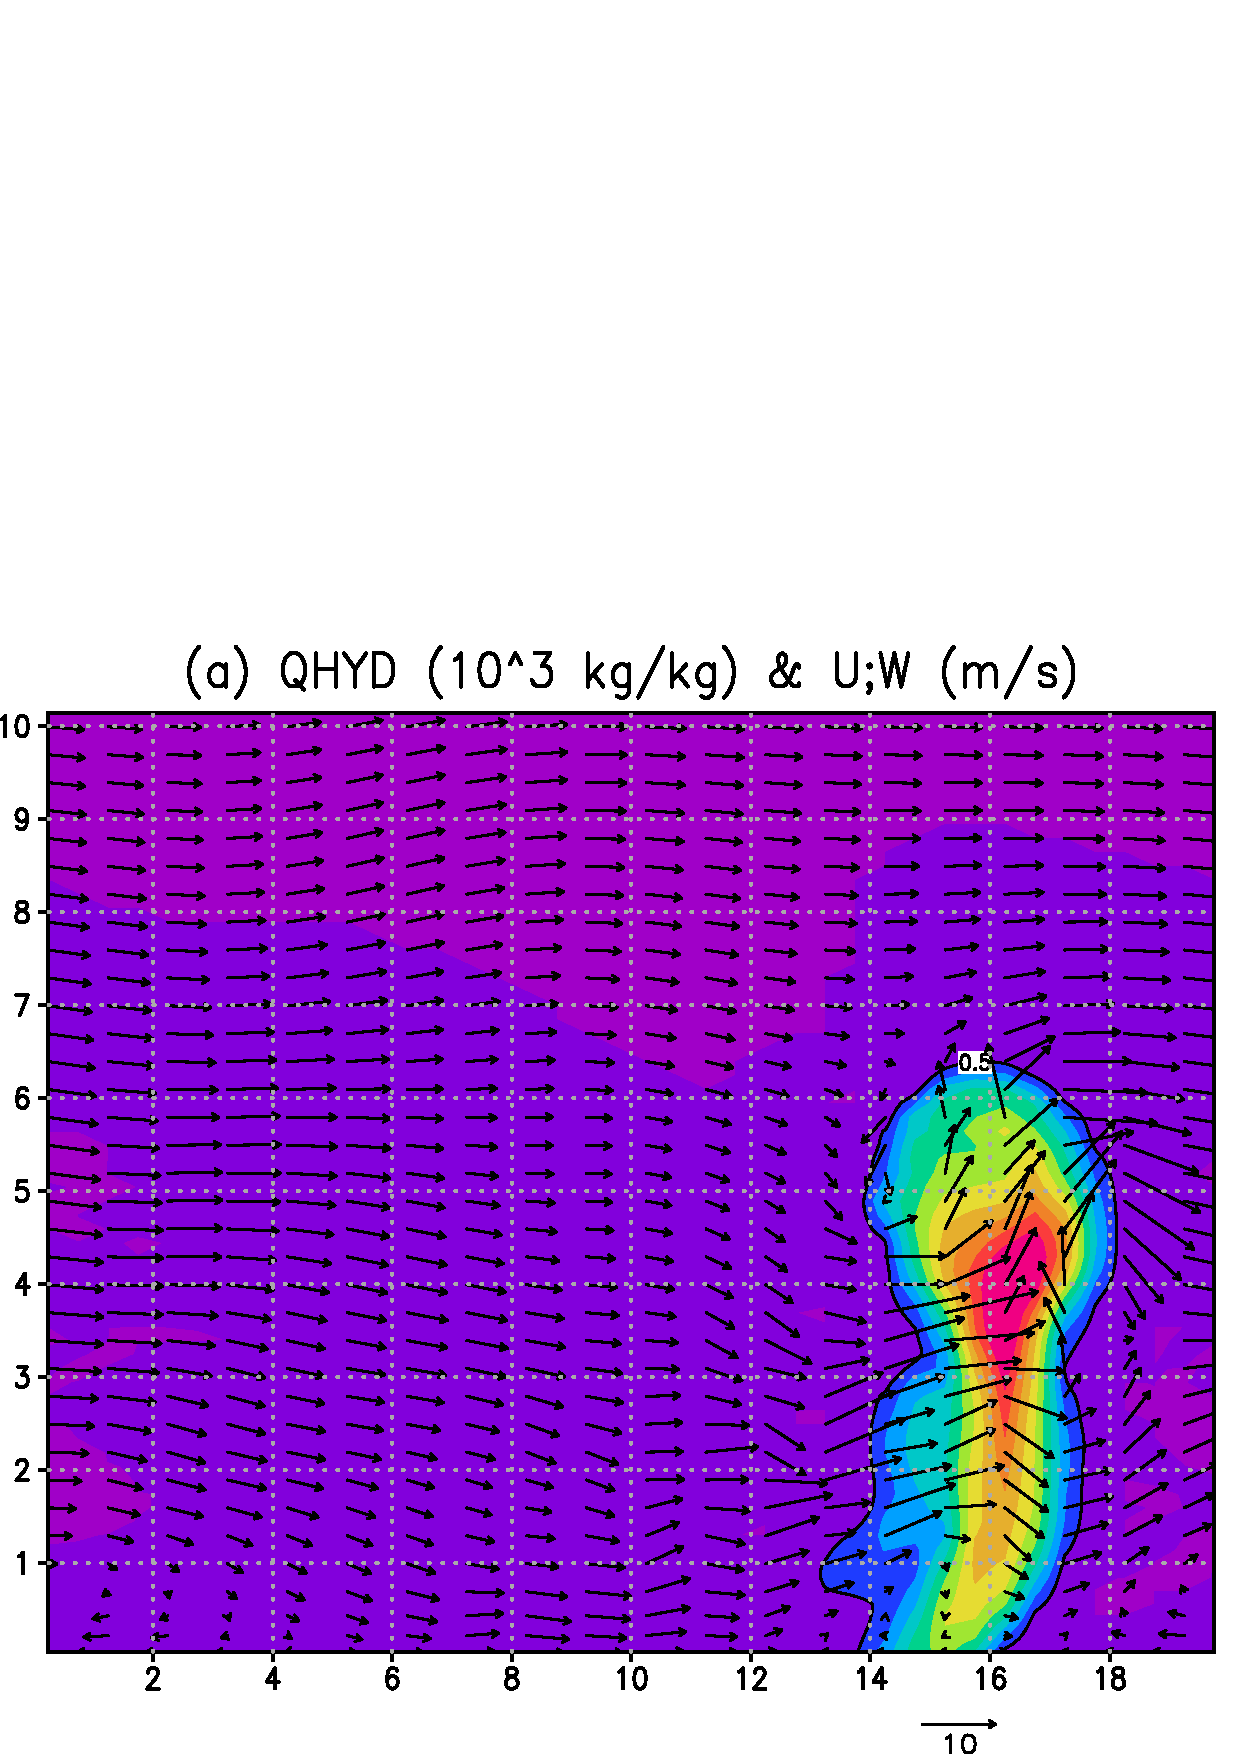
\includegraphics[width=0.7\hsize]{./../../figure/ideal_qhyd.pdf}\\
  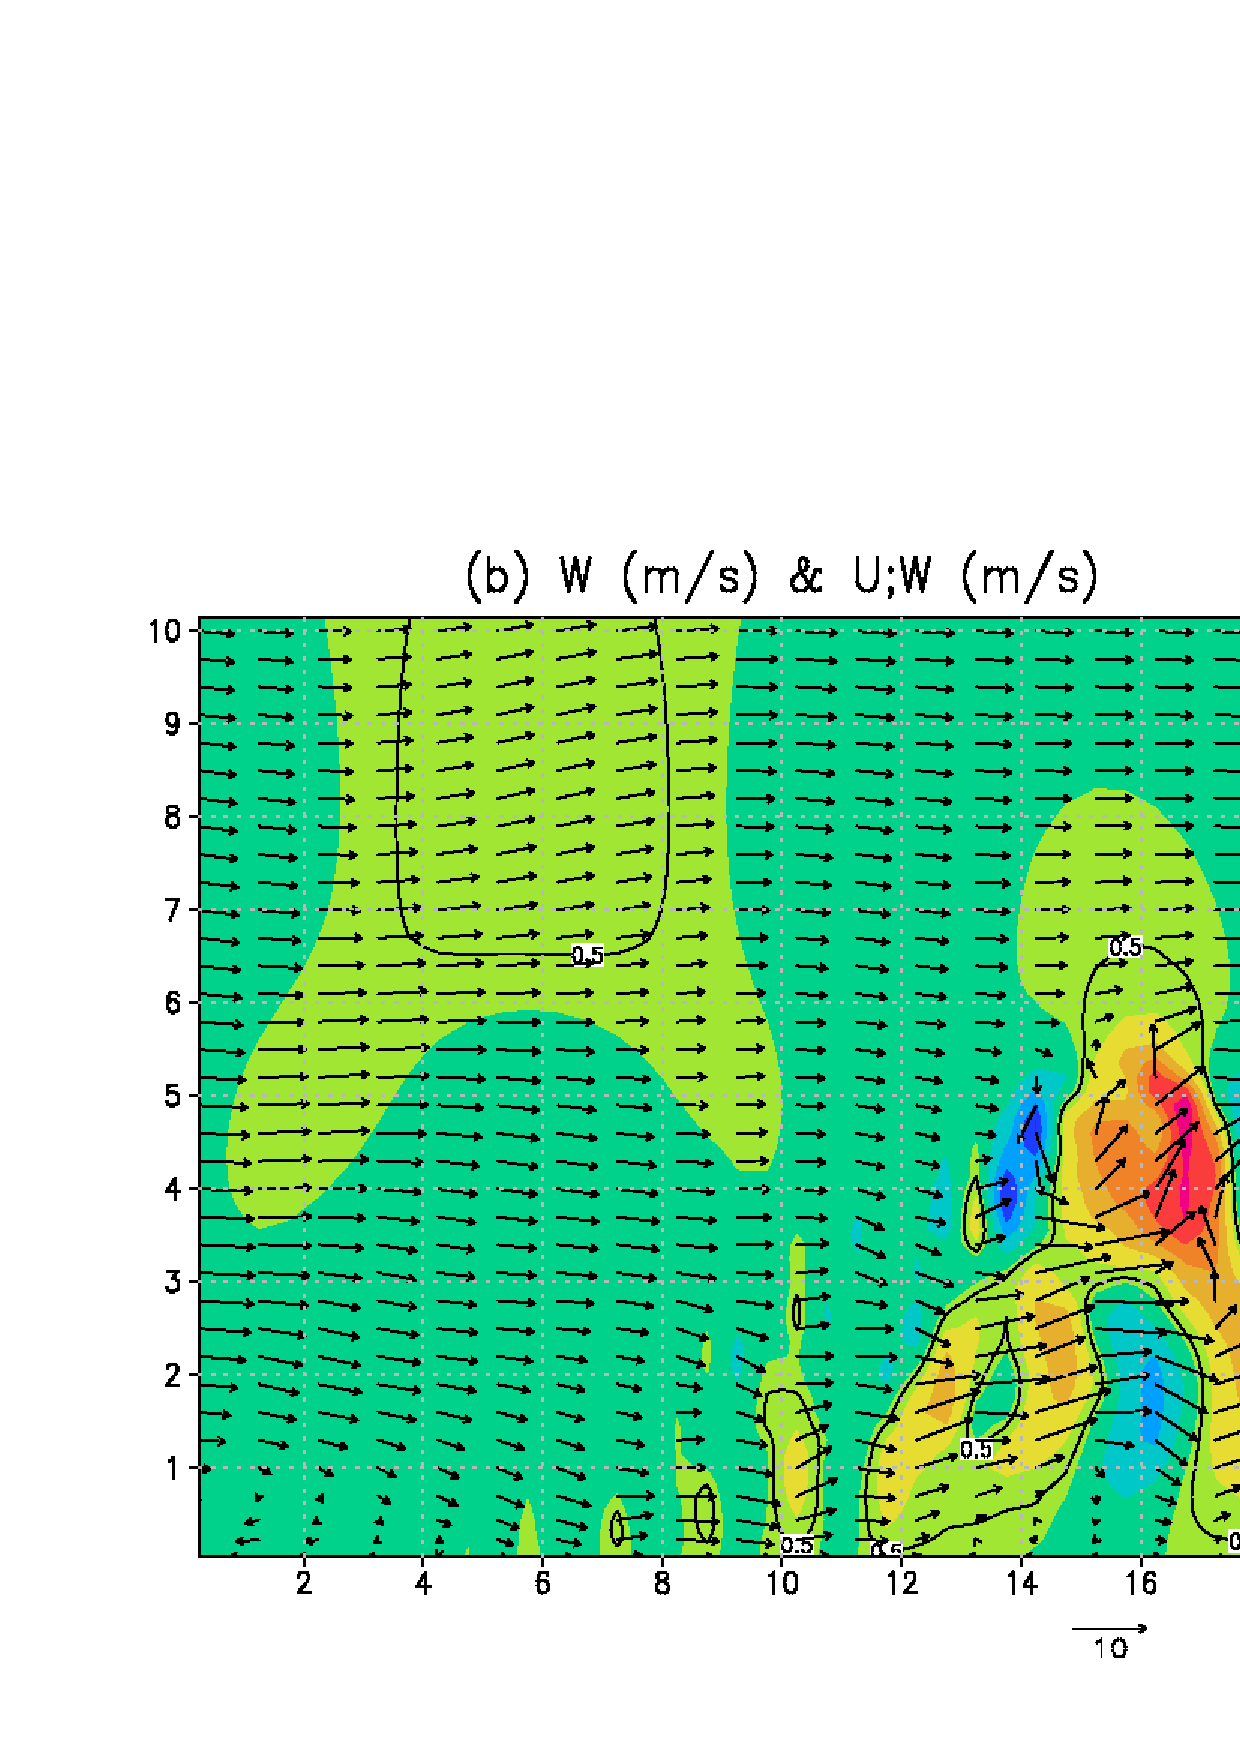
\includegraphics[width=0.7\hsize]{./../../figure/ideal_W.pdf}\\
  \caption{積分開始から 1200 秒(20 分)後の水平-鉛直断面図;
           図(a)に全質量に対する凝結物の質量比、図(b)に鉛直速度を示す。
           両方の図において、ベクトルは流れを表す。}
  \label{fig_ideal}
\end{center}
\end{figure}

ヒストリファイルに出力された変数は、{\netcdf} の\verb|ncdump| 等を用いて簡単に確認できる。
\sno の詳しい使い方は第\ref{sec:sno}節を参照されたい。
